\documentclass{article}
%% Cover by Bart Snapp

\usepackage{tikz} 
\usepackage{pgfplots} 
\usepackage{stix}
\usepackage{gillius}
\usepackage{ccicons}

\usepackage[margin=0in, includehead, includefoot, paperwidth=8.625in, paperheight=8.75in]{geometry}
\usetikzlibrary{backgrounds}
\usetikzlibrary{patterns}


\definecolor{scarlet}{RGB}{187,0,0}

\begin{document}
\pagenumbering{gobble}


\tikz[remember picture,overlay] \node[inner sep=0pt] at (current page.center){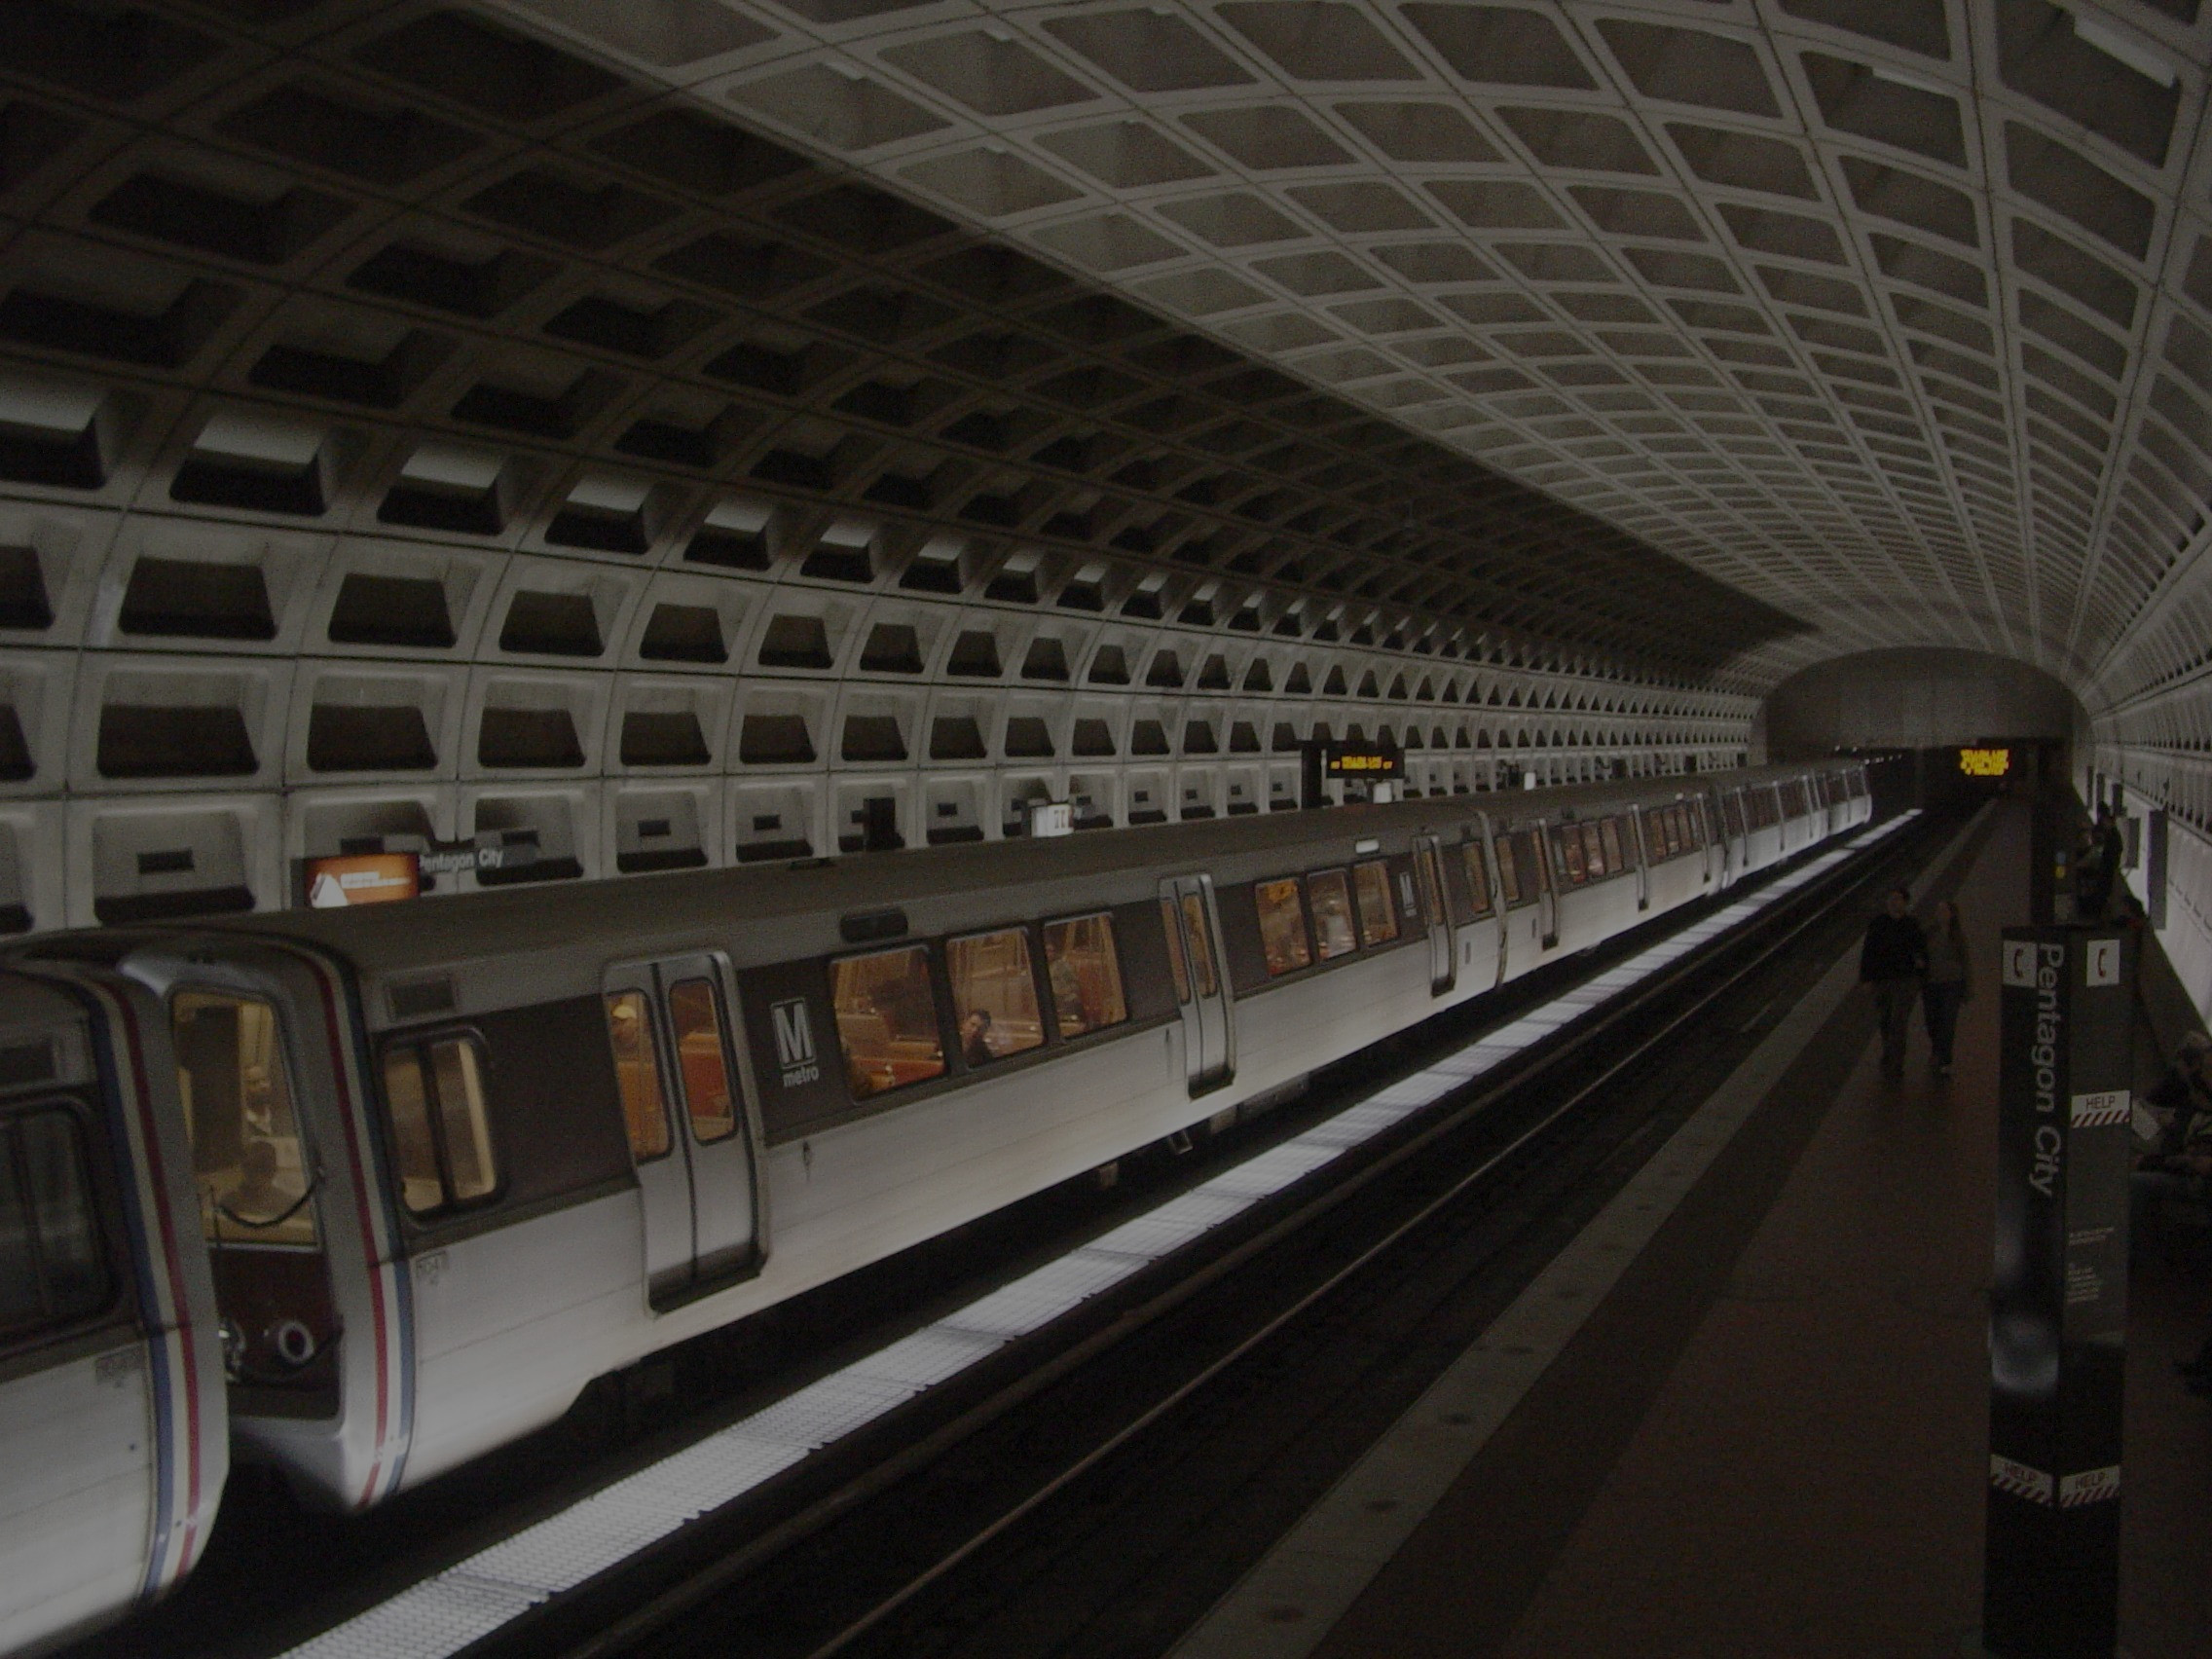
\includegraphics[height=8.75in]{metroStationDark.jpg}};
%\tikz[remember picture,overlay] \node[inner sep=0pt] at (current page.center){\includegraphics[width=8.625in]{frontTemplate.png}};

\flushright
\begin{tikzpicture}[opacity=1]
  \node at (-2.3,0) {\scalebox{3}{\Huge\textsf{\textbf{\textcolor{white}{linear algebra}}}}};
  %% \node at (8,1.19) {\scalebox{7}{\Huge\textsf{\textbf{\textcolor{white!65!black}{\&}}}}};  %% Aligned with subtitle
  %% \node[right] at (-3,-2.4) {\scalebox{3}{\Huge\textsf{\textbf{\textcolor{white}{ordinary}}}}};
  %% \node[right]at (-3,-4.5) {\scalebox{3}{\Huge\textsf{\textbf{\textcolor{white}{differential}}}}};
  %% \node[right] at (-3,-6.8) {\scalebox{3}{\Huge\textsf{\textbf{\textcolor{white}{equations}}}}};
  %% %\node at (8,1.85) {\scalebox{10}{\Huge\textsf{\textbf{\textcolor{white!65!black}{1}}}}}; %% Aligned with title
  \node[right] at (-3,-8.2){\resizebox{4.8in}{.2in}{\Huge\textsf{\textcolor{white!65!black}
          {with free online interactive materials}
    }}};
    %\draw[yellow] (-9,-1.2)--(9,-1.2); %guide line
\end{tikzpicture}\hspace*{.3in}
\vfill

\flushleft
\hspace*{.4in}\begin{tikzpicture}
  \node at (0,0) {\scalebox{1}{\Huge\textsf{\textcolor{white}{\ccbyncsa}}}};
  \node at (4,-.2) {\large\textsf{\textcolor{white}{developed in \textbf{XIMERA}}}};
  \node[right] at (4,1) {\Huge\textsf{\textcolor{white}{Martin Golubitsky and Michael Dellnitz}}};
\end{tikzpicture}
\vspace*{.2cm}

\end{document}


